\documentclass[11pt]{article} 
\usepackage{calc, tikz}
\usepackage[margin={1in,1in}]{geometry} 
\usepackage[hwkhandout]{hwk}
\usepackage[pdftitle={Calc 1
  Notes},colorlinks=true,urlcolor=blue]{hyperref}

\renewcommand{\theclass}{\textsc{math}1300: calculus I}
\renewcommand{\theauthor}{Tyson Gern}
\renewcommand{\theassignment}{Parametric Equations}
\renewcommand{\dateinfo}{section 4.8}

\newcommand{\ds}{\displaystyle}

\begin{document}
\drawtitle

\begin{enumerate}

\item Write the parameterizations of the following lines.
  \begin{enumerate}
  \item The line through the points $(2,-1)$ and $(1,3)$
    \vfill
  \item A horizontal line through the point $(2, 8)$
    \vfill
  \item A vertical line through the point $(-4, 7)$
    \vfill
  \item The line $y=7x-14$
    \vfill
  \end{enumerate}
  \newpage

\item Describe the motion of a particle moving according to the given
  parametric equations, and find the equation of the curve along which
  the particle moves.
  
  \begin{enumerate}
  \item 
    \begin{align*}
      x(t) &= t - 9\\
      y(t) &= 9 - 3t.
    \end{align*}
    \vfill
  \item
    \begin{align*}
      x(t) &= 2\cos(-t)\\
      y(t) &= 3\sin(-t).
    \end{align*}
    \vfill
  \end{enumerate}
  \newpage
  
\item The motion of a particle on the $xy$-plane is given by
  \begin{align*}
    x(t) &= t^3 - \frac{3}{2}t^2 - 6t\\
    y(t) &= t^3 - \frac{9}{2}t^2 + 6t.\\
  \end{align*}

  \begin{enumerate}
  \item Does the particle ever come to a complete stop?  If so, when
    and where?
    \vfill
  \item Is the particle ever moving straight up or down?  If so, when
    and where?
    \vfill
  \item Is the particle ever moving straight horizontally right or
    left?  If so, when and where?
    \vfill
  \end{enumerate}
  \newpage
  
\item Two particles move in the $xy$-plane.  At time $t$, the position
  of a particle $A$ is given by
  \begin{align*}
    x(t) &= 4t - 4\\
    y(t) &= 2t - k,\\
    \intertext{and the position of particle $B$ is given by}
    x(t) &= 3t\\
    y(t) &= t^2 - 2t - 1.
  \end{align*}

  \begin{enumerate}
  \item If $k=5$ do the particles ever collide?  Explain.
    \vfill
  \item Find $k$ so that the two particles do collide.
    \vfill
  \item At the time that the particles collide in part (b), which
    particle is moving faster?
    \vfill
  \end{enumerate}
  \newpage

\item The figure below shows the graph of the parametric curve
  \begin{align*}
    x(t) &= f(t)\\
    y(t) &= f'(t),
  \end{align*}
  for a function $f(t)$.
    \begin{center}
      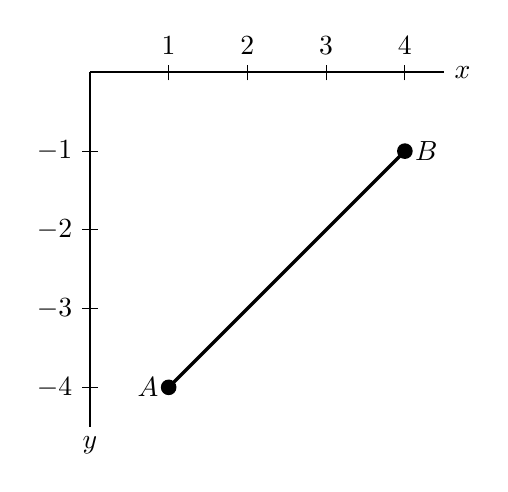
\begin{tikzpicture}
        \def\xmin{-0}\def\xmax{5} \def\ymin{-5}\def\ymax{0} 
        \foreach \i in {\xmin,...,4} {\ifnum\i=0{}
          \else{\draw
            (\i,-.1) -- (\i,.1) node[above] {$\i$};}\fi}
        \foreach \i in {-4,...,\ymax} {\ifnum\i=0{}
          \else{\draw
            (.1, \i) -- (-.1, \i) node[left] {$\i$};}\fi}
        
        \draw[thick] (\xmin,0) -- (4.5,0) node[right] {$x$}; \draw[thick] (0,0) --
        (0,-4.5) node[below] {$y$};
        
        \draw[very thick] (1,-4) -- (4,-1);
        \draw [thick, fill=black] (1,-4) circle [radius=0.085] node[left]{$A$};
        \draw [thick, fill=black] (4,-1) circle [radius=0.085] node[right]{$B$};
    \end{tikzpicture}
  \end{center}

  \begin{enumerate}
  \item Is $f(t)$ an increasing or decreasing function?
    \vfill
  \item As $t$ increases, is the curve traced from $A$ to $B$ or from
    $B$ to $A$?
    \vfill
  \item Is $f(t)$ concave up or concave down?
    \vfill
  \end{enumerate}


\end{enumerate}

\end{document}
